\section*{page 21}

\underline{child convergence} assume during concurrent learning\\

\begin{itemize}
\item $R_t$ must be time-monotonic and convergent stochastic.\\
\item Evaluate selection of $s^\prime_i$ and $s_i$, assuming worst case: $a_k$ has no impact on $s^\prime_k$, $s_k$ and only an impact on $s_i$ and $s^\prime_i$\\
\begin{center}
\scalebox{0.5}{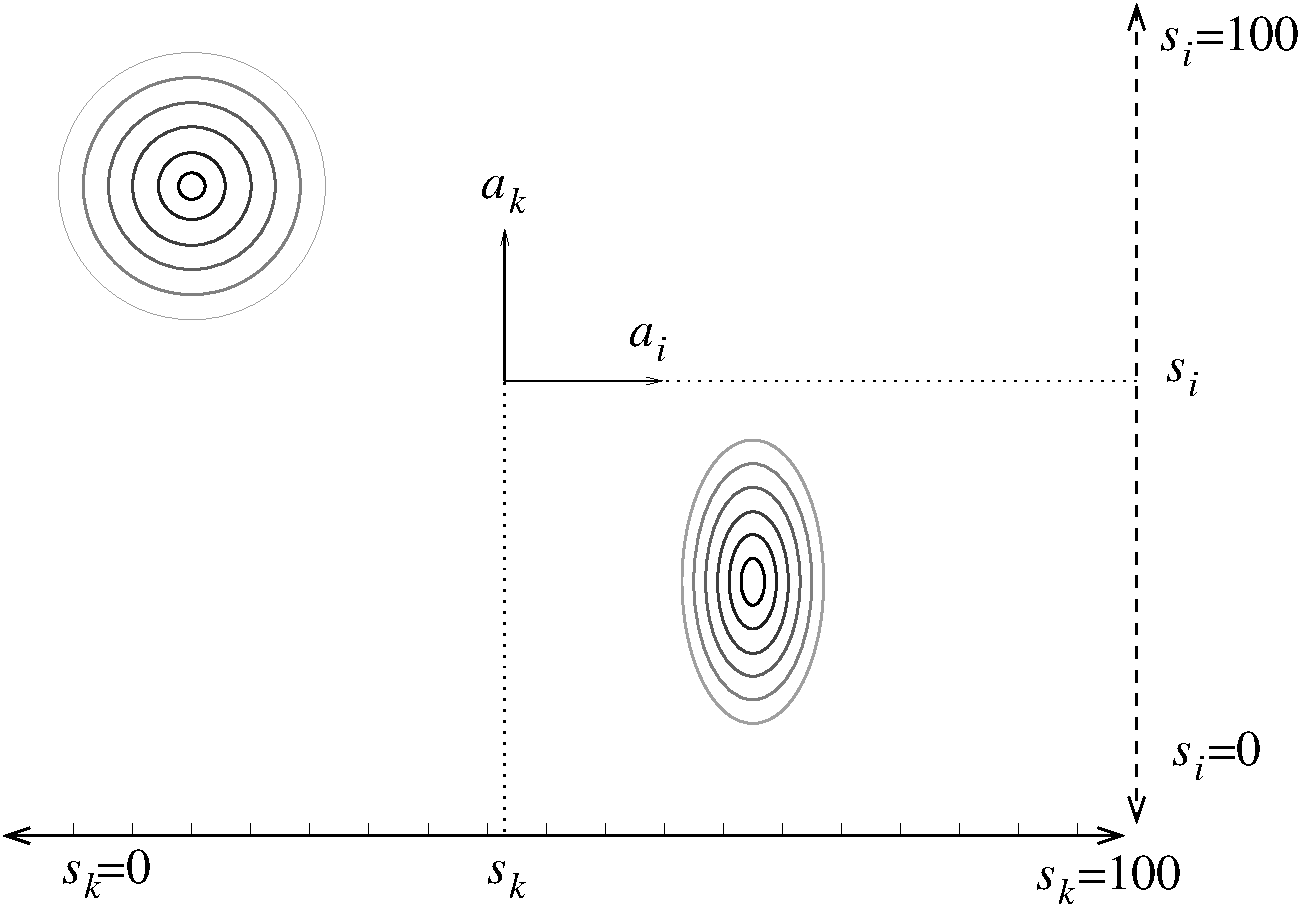
\includegraphics{media/page21figure}}
\end{center}
consider policy learning: execution of $\pi_k(s_k)$ yielding $s^\prime_k$
\end{itemize}

\setlength{\unitlength}{1cm}
\begin{picture}(15,15)
\put(7.5,14.7){choice of $a_k$}
\put(8.3,14.25){\vector(-1,-1){3.0}}
\put(8.3,14.25){\vector(1,-1){3.0}}
\put(5.65,13.4){good}
\put(5.65,12.9){$s_i$, $s_j$}
\put(6.7,12.1){$a_k\in\text{Good}$}
\put(6.2,11.5){\underline{$Q(s_k,a_{k1})$}}
%
\put(4.1,10.3){$M_i$}
\put(3.9,9.65){\vector(-1,-1.2){2.0}}
\put(4.6,9.65){\vector(1,-1.2){2.0}}
%
\put(1.7,8.5){same}
\put(1.65,6.5){\circled{A}}
\put(0.8,5.5){$R_t()$ stays same}
%
\put(5.9,8.5){improves}
\put(6.45,6.5){\circled{B}}
\put(5.8,5.5){$R_t()$ increases}
%
\put(9.8,13.4){bad}
\put(9.8,12.9){$s_i$, $s^\prime_i$}
\put(8.8,12.1){$a_k\in\text{Bad}$}
\put(9,11.5){\underline{$Q(s_k,a_{k2})$}}
%
%
\put(10.5,10.3){$M_i$ chooses $a_i$ (store $s_i$, $s_j$, $a_k$)}
\put(11.7,9.65){\vector(-1,-1.2){2.0}}
\put(12.4,9.65){\vector(1,-1.2){2.0}}
%
\put(9,8.5){stays bad}
\put(9.5,6.5){\circled{C}}
\put(8.5,5.5){\parbox[t]{2.5cm}{$M_i$ can't learn to improve situation}}
\put(8.5,4){$R_t()\text{s}$ stagnate}
%
\put(13.9,8.5){turns max Q(}
\put(14.5,6.5){\circled{D}}
\put(13.5,5.5){\parbox[t]{2.5cm}{$M_i$ learning to create maximum reward using $a_i$}}
\put(13.5,4){$R_t()$ increases}
%
\qbezier(2,3)(2.4,1.4)(4,1)
\qbezier(6,3)(6.3,1.8)(7,1)
\qbezier(10,3)(9.7,1.8)(9,1)
\qbezier(14.5,3)(14.1,1.4)(12.5,1)
\put(6,0){end up in same $s_k^\prime=s_k$, so complete degeneracy}
\end{picture}

As $t\to\infty$,\begin{minipage}[t]{\linegoal} 
\begin{enumerate}[label=\roman*)]
\item \circled{A} \& \circled{C} will never be selected by $M_k()$
\item if \circled{B}$>$\circled{D} $Q(a_k\in\text{Good},s_k)>Q(a_k\in\text{Bad})$ and then $a_k\in\text{Good}$ will be chosen
\end{enumerate}
\end{minipage}